% Historical milestones, not an exhaustive chapter chronology.
\begin{frame}{San Francisco: overlapping communities, future founders}
  \begin{columns}[c,onlytextwidth]
    \column{.56\textwidth}
      \small
      \NTXPoint{Dream Team at Noisebridge}{I collaborated with the Dream Team and other groups forming around neurotech.}
      \NTXPoint{OpenBCI contributors to Neurosity founders}{AJ Keller / Push The World and Alex Castillo contributed firmware, drivers, and JavaScript tools before Neurosity.}
      \NTXPoint{Connections cross city boundaries}{AJ discovered OpenBCI through NeuroTechX; he and Alex met at a New York hackday in 2016.}
    \column{.40\textwidth}
      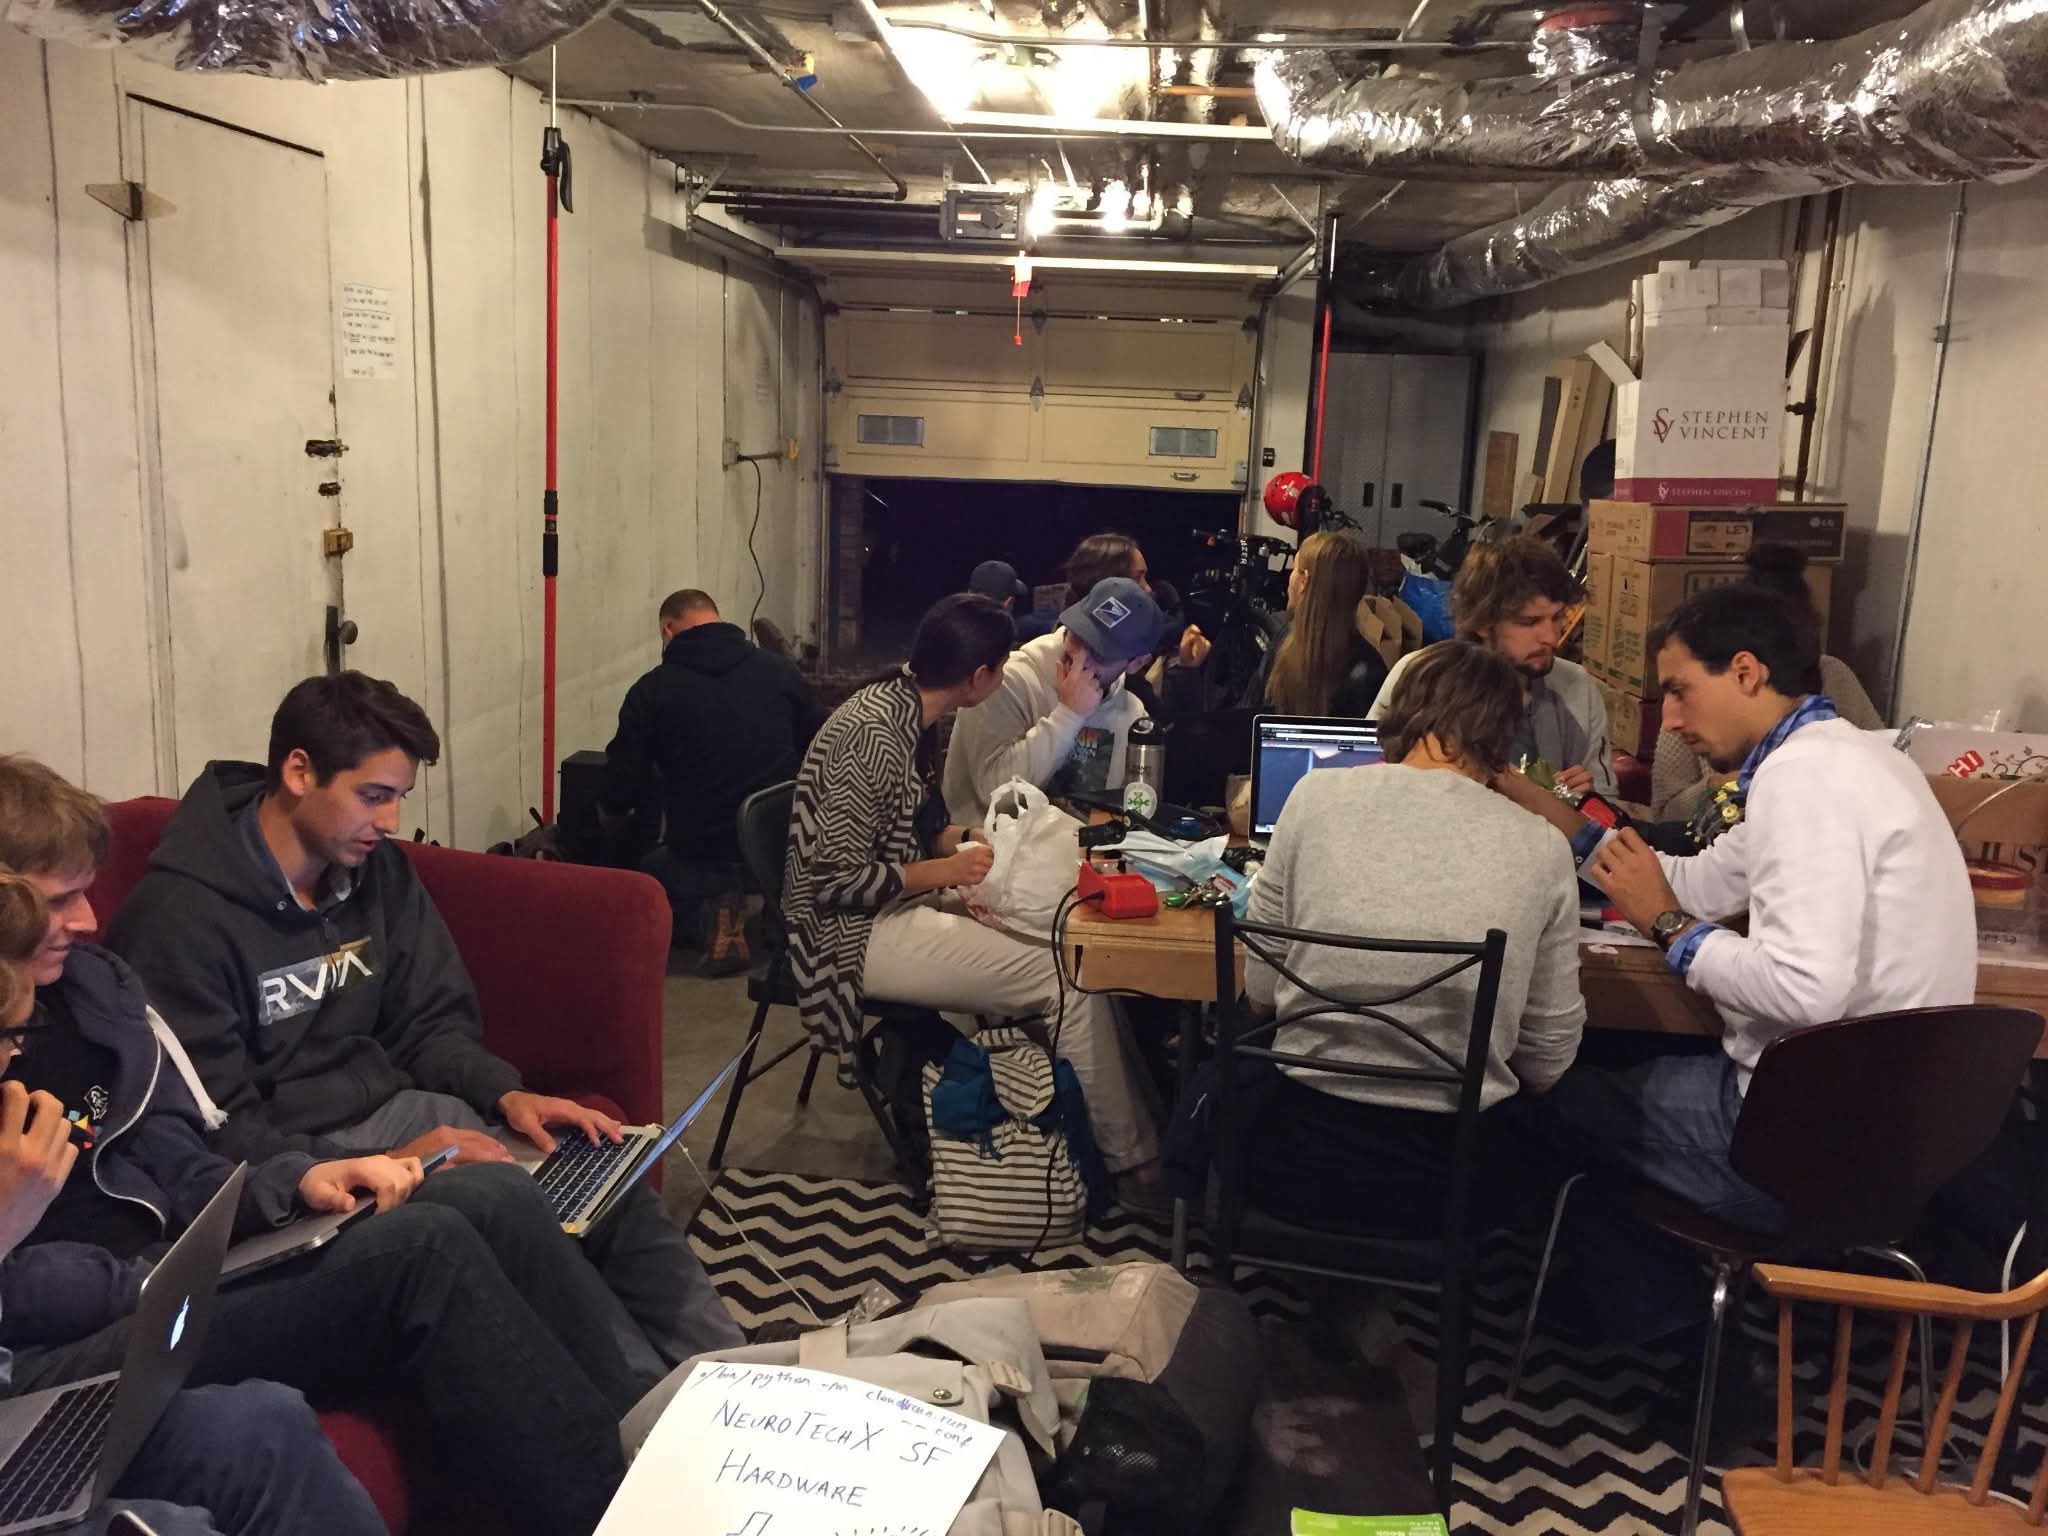
\includegraphics[width=\linewidth,height=39mm,keepaspectratio]{assets/chapters/san-francisco-original-hacknight.jpg}\par\smallskip
      {\tiny Original SF Hacknights / Morgan Hough\newline Community context, not a Dream Team event photo\par}
  \end{columns}
  {\tiny\color{NTXMuted}Sources: \href{https://www.noisebridge.net/wiki/DreamTeam}{DreamTeam}; \href{https://openbci.com/community/openbci-and-push-the-world/}{AJ Keller}; \href{https://openbci.com/community/new-javascript-open-source-projects-for-openbci/}{Alex Castillo, 2017}; \href{https://neurosity.co/about}{Neurosity}. Personal collaborations: Morgan Hough.\par}
  \note{[08:15--09:15] Morgan identifies his collaboration with the Dream Team at Noisebridge and other neurotech groups, and places Neurosity in his San Francisco ecosystem account. Noisebridge's indexed wiki describes DreamTeam as a neurohacking and AI experimentation group and lists OpenBCI, OpenEEG and other devices. AJ's OpenBCI guest post says he discovered OpenBCI through NeuroTechX. His later first-person account dates meeting Alex at an OpenBCI Friday hackday to 2016 and their shared Neurosity idea to 2018. OpenBCI's 2016 and 2017 records document Push The World's firmware and driver work; Alex's December 2017 JavaScript post thanks AJ. Distinguish New York origins of that collaboration from the later SF connection. No claim that Neurosity founded OpenBCI, that all named groups merged into NTX, or that Morgan collaborated personally with every founder. The photo is the existing SF Hacknight image, not identified as DreamTeam.}
\end{frame}

\begin{frame}{Toronto: learning together, building open tools}
  \begin{columns}[c,onlytextwidth]
    \column{.52\textwidth}
      \small
      \NTXPoint{Local roots: Steve Mann and InteraXon}{U of T's wearable and thought-controlled computing work; Ariel Garten's connection to Mann helped shape InteraXon's origins.}
      \NTXPoint{2016: learning and building together}{EEG lectures and biweekly Hacknights; open projects including EEG 101 and Neurodoro, in an ecosystem connected to InteraXon.}
      \NTXPoint{Student builders}{NeuroTechUofT's 2016 demo: VitReous, an eye-gesture interface for VR/AR.}
    \column{.43\textwidth}
      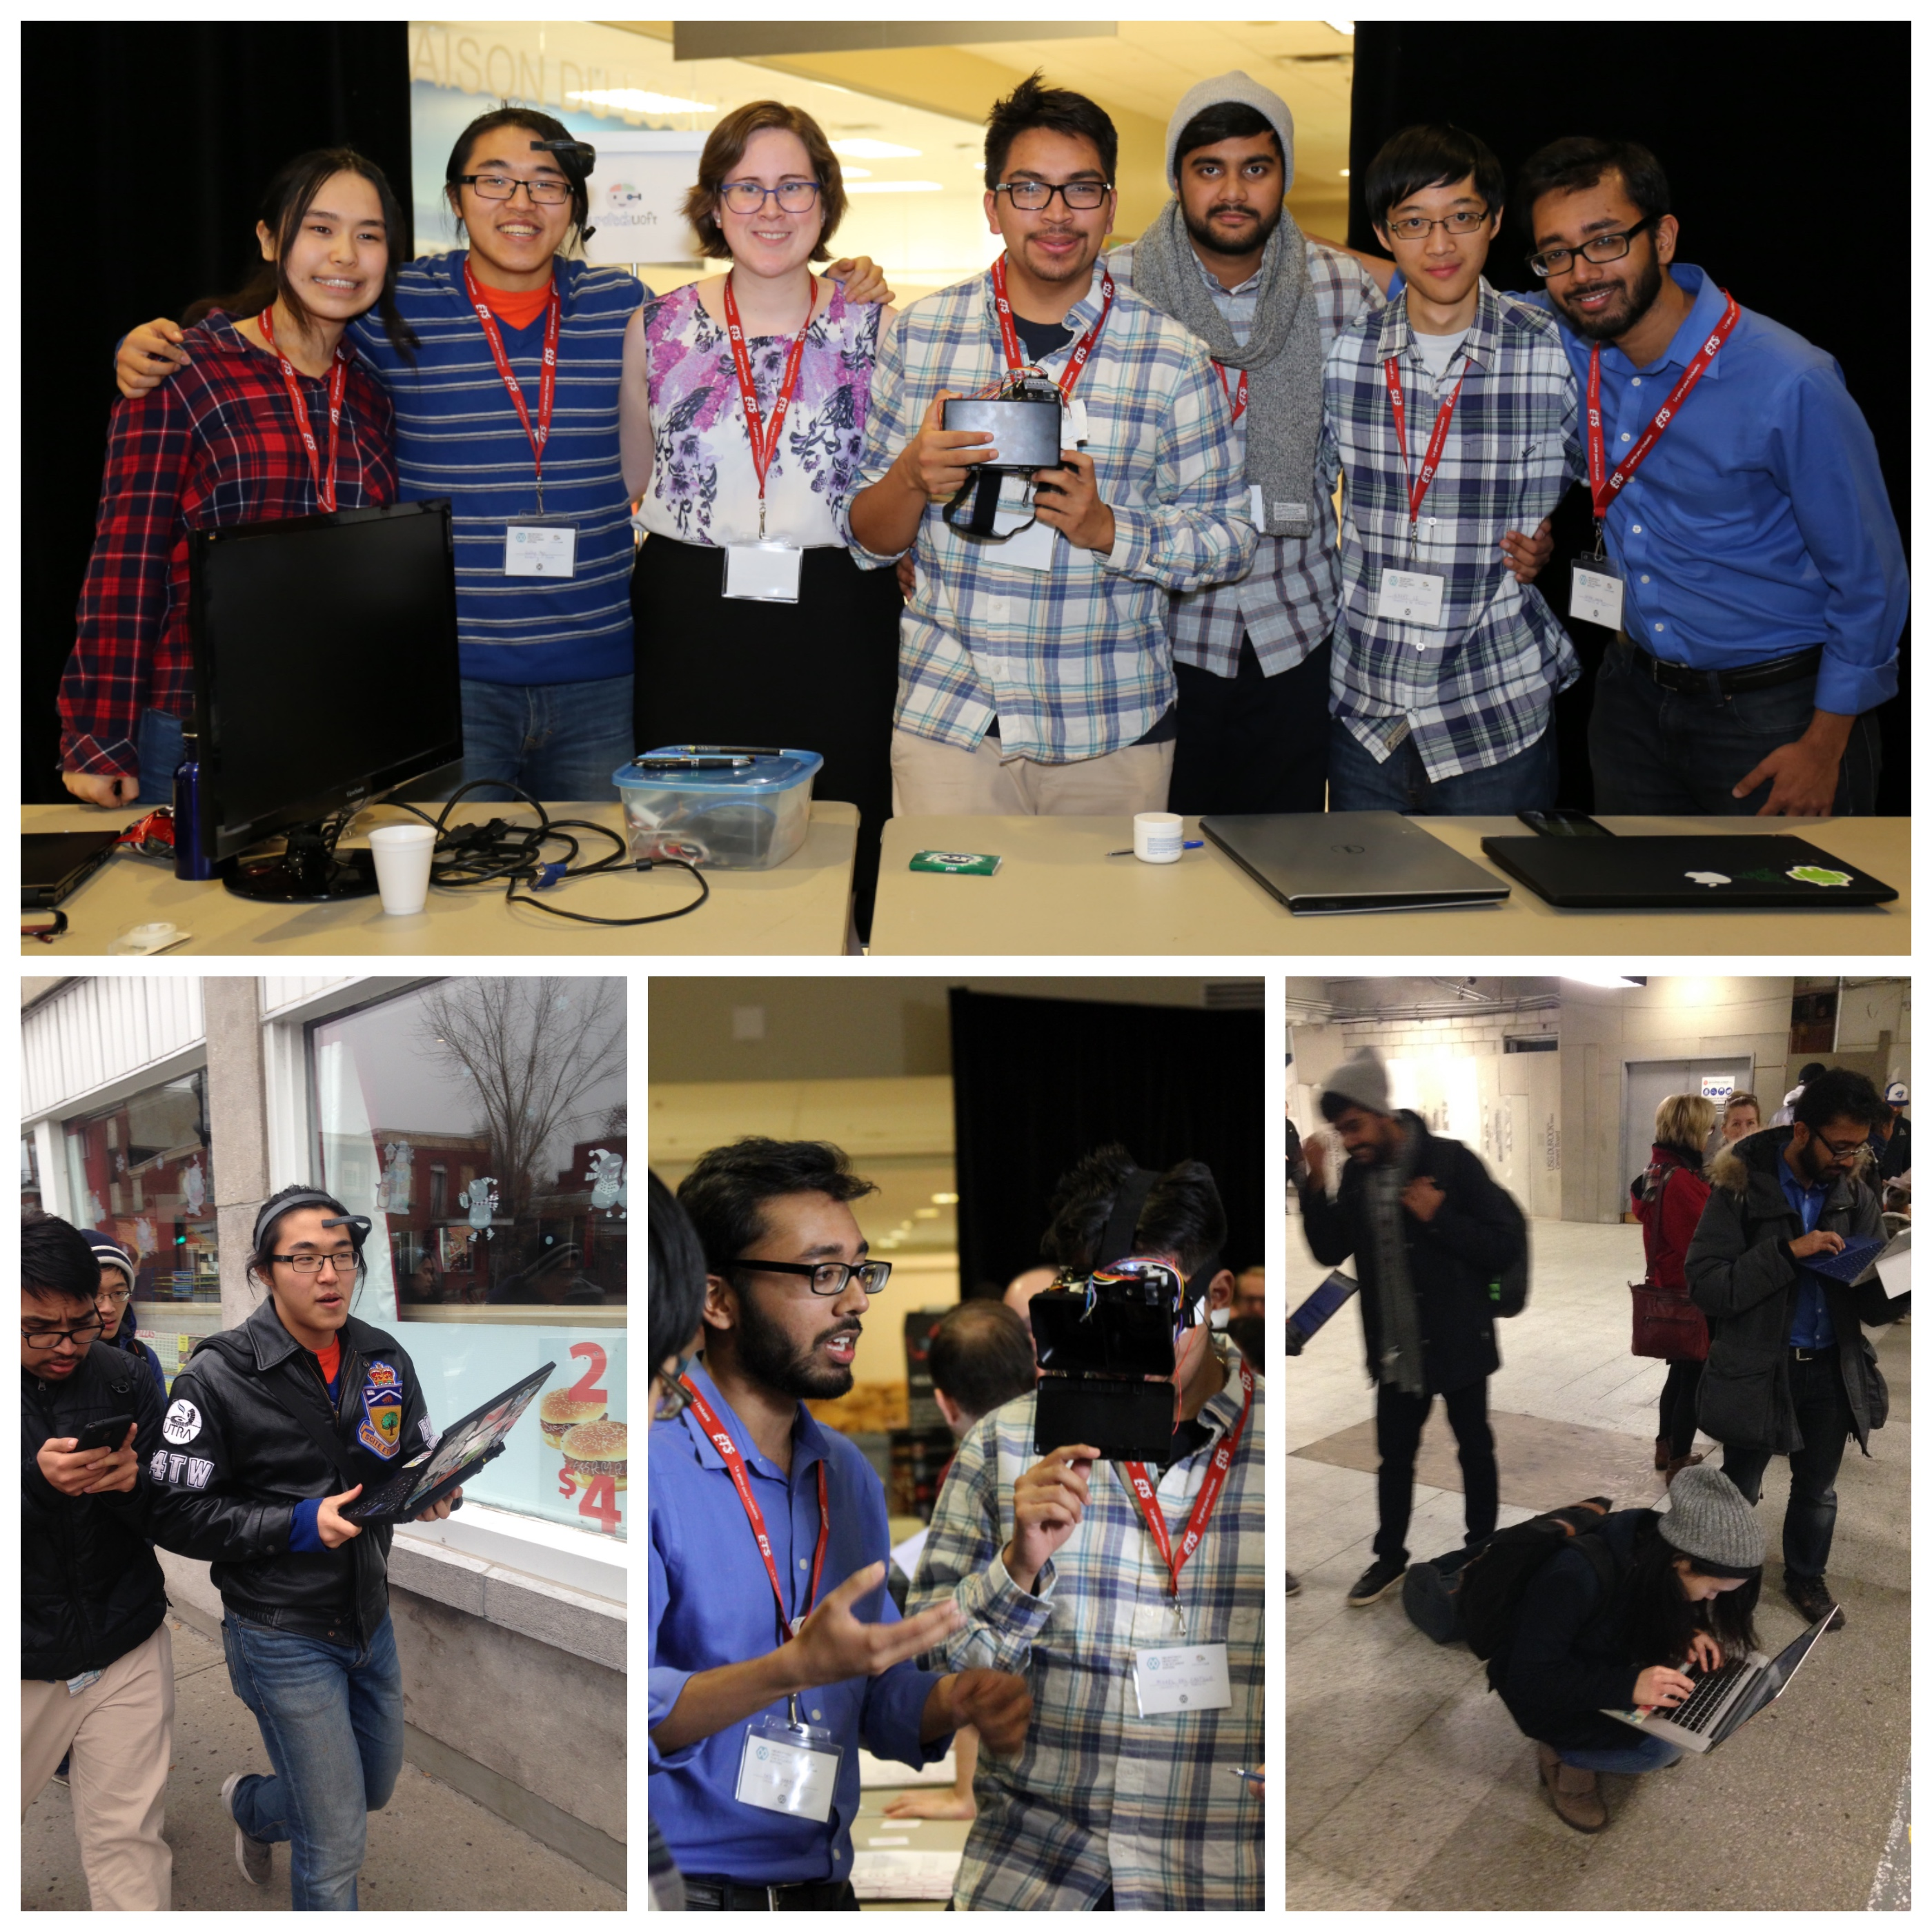
\includegraphics[width=\linewidth,height=48mm,keepaspectratio]{assets/chapters/toronto-student-demo-2016.jpg}
      \par\smallskip{\scriptsize NeuroTechUofT --- Student Demo Day, 2016\par}
  \end{columns}
  {\tiny\color{NTXMuted}Sources: \href{https://news.engineering.utoronto.ca/thought-control-technology-can-make-toast/}{U of T, 2010}; \href{https://www.ece.utoronto.ca/people/mann-s/}{Steve Mann}; \href{https://neurotechx.com/chapter/1531/}{Toronto chapter}; \href{https://neurotechx.github.io/studentclubs/news/student-clubs-2016/}{student archive / photo}\par}
  \note{[09:15--10:15] Toronto's community sits in a longer local history. U of T's August 2010 account connects InteraXon CEO Ariel Garten with her former teacher Steve Mann and his thought-controlled computing work. Mann's faculty profile documents his wearable-computing and EyeTap research. Distinguish this technology lineage from the chapter's own founding: neither Mann nor InteraXon is asserted to have founded NTX Toronto. The chapter archive names connections with InteraXon, Avertus and the Ontario Brain Institute, and describes biweekly Hacknights and open mobile projects. The February 2016 NTX Digest records January's EEG lectures. The image is NeuroTechUofT's 2016 student Demo Day, not a Mann or InteraXon demonstration. VitReous used EOG eye gestures, not EEG decoding. EEG 101 is historical: its repository was archived in 2021 after loss of Muse SDK support. The lesson is the interplay of university research, local companies, and community-led learning.}
\end{frame}

\begin{frame}{New York: from Hacknights to NeuroNYC meetings}
  \begin{columns}[c,onlytextwidth]
    \column{.52\textwidth}
      \small
      \NTXPoint{2015: an early NeuroTechX community}{Conor Russomanno's organizing history begins in July; monthly Hacknights around human--computer interfaces.}
      \NTXPoint{2016: prototype testing together}{Dark Maze was tested at a NeuroTechNYC meetup using OpenBCI.}
      \NTXPoint{2025--26: NeuroNYC meetings}{Happy hours, NeuroBall, a summer summit, and a foundation-models symposium connect today's ecosystem.}
    \column{.43\textwidth}
      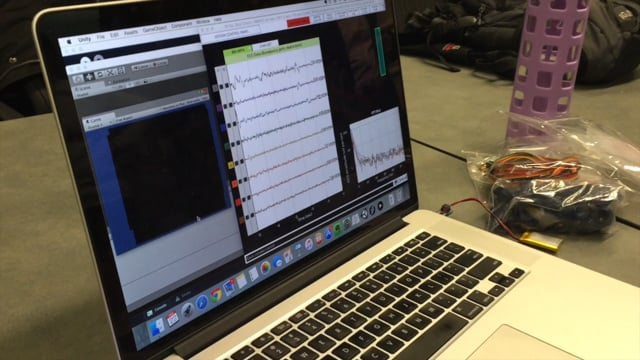
\includegraphics[width=\linewidth,height=23mm,keepaspectratio]{assets/chapters/new-york-darkmaze-2016.jpg}
      \par{\tiny Dark Maze meetup test, 2016 / Mathura\par}\smallskip
      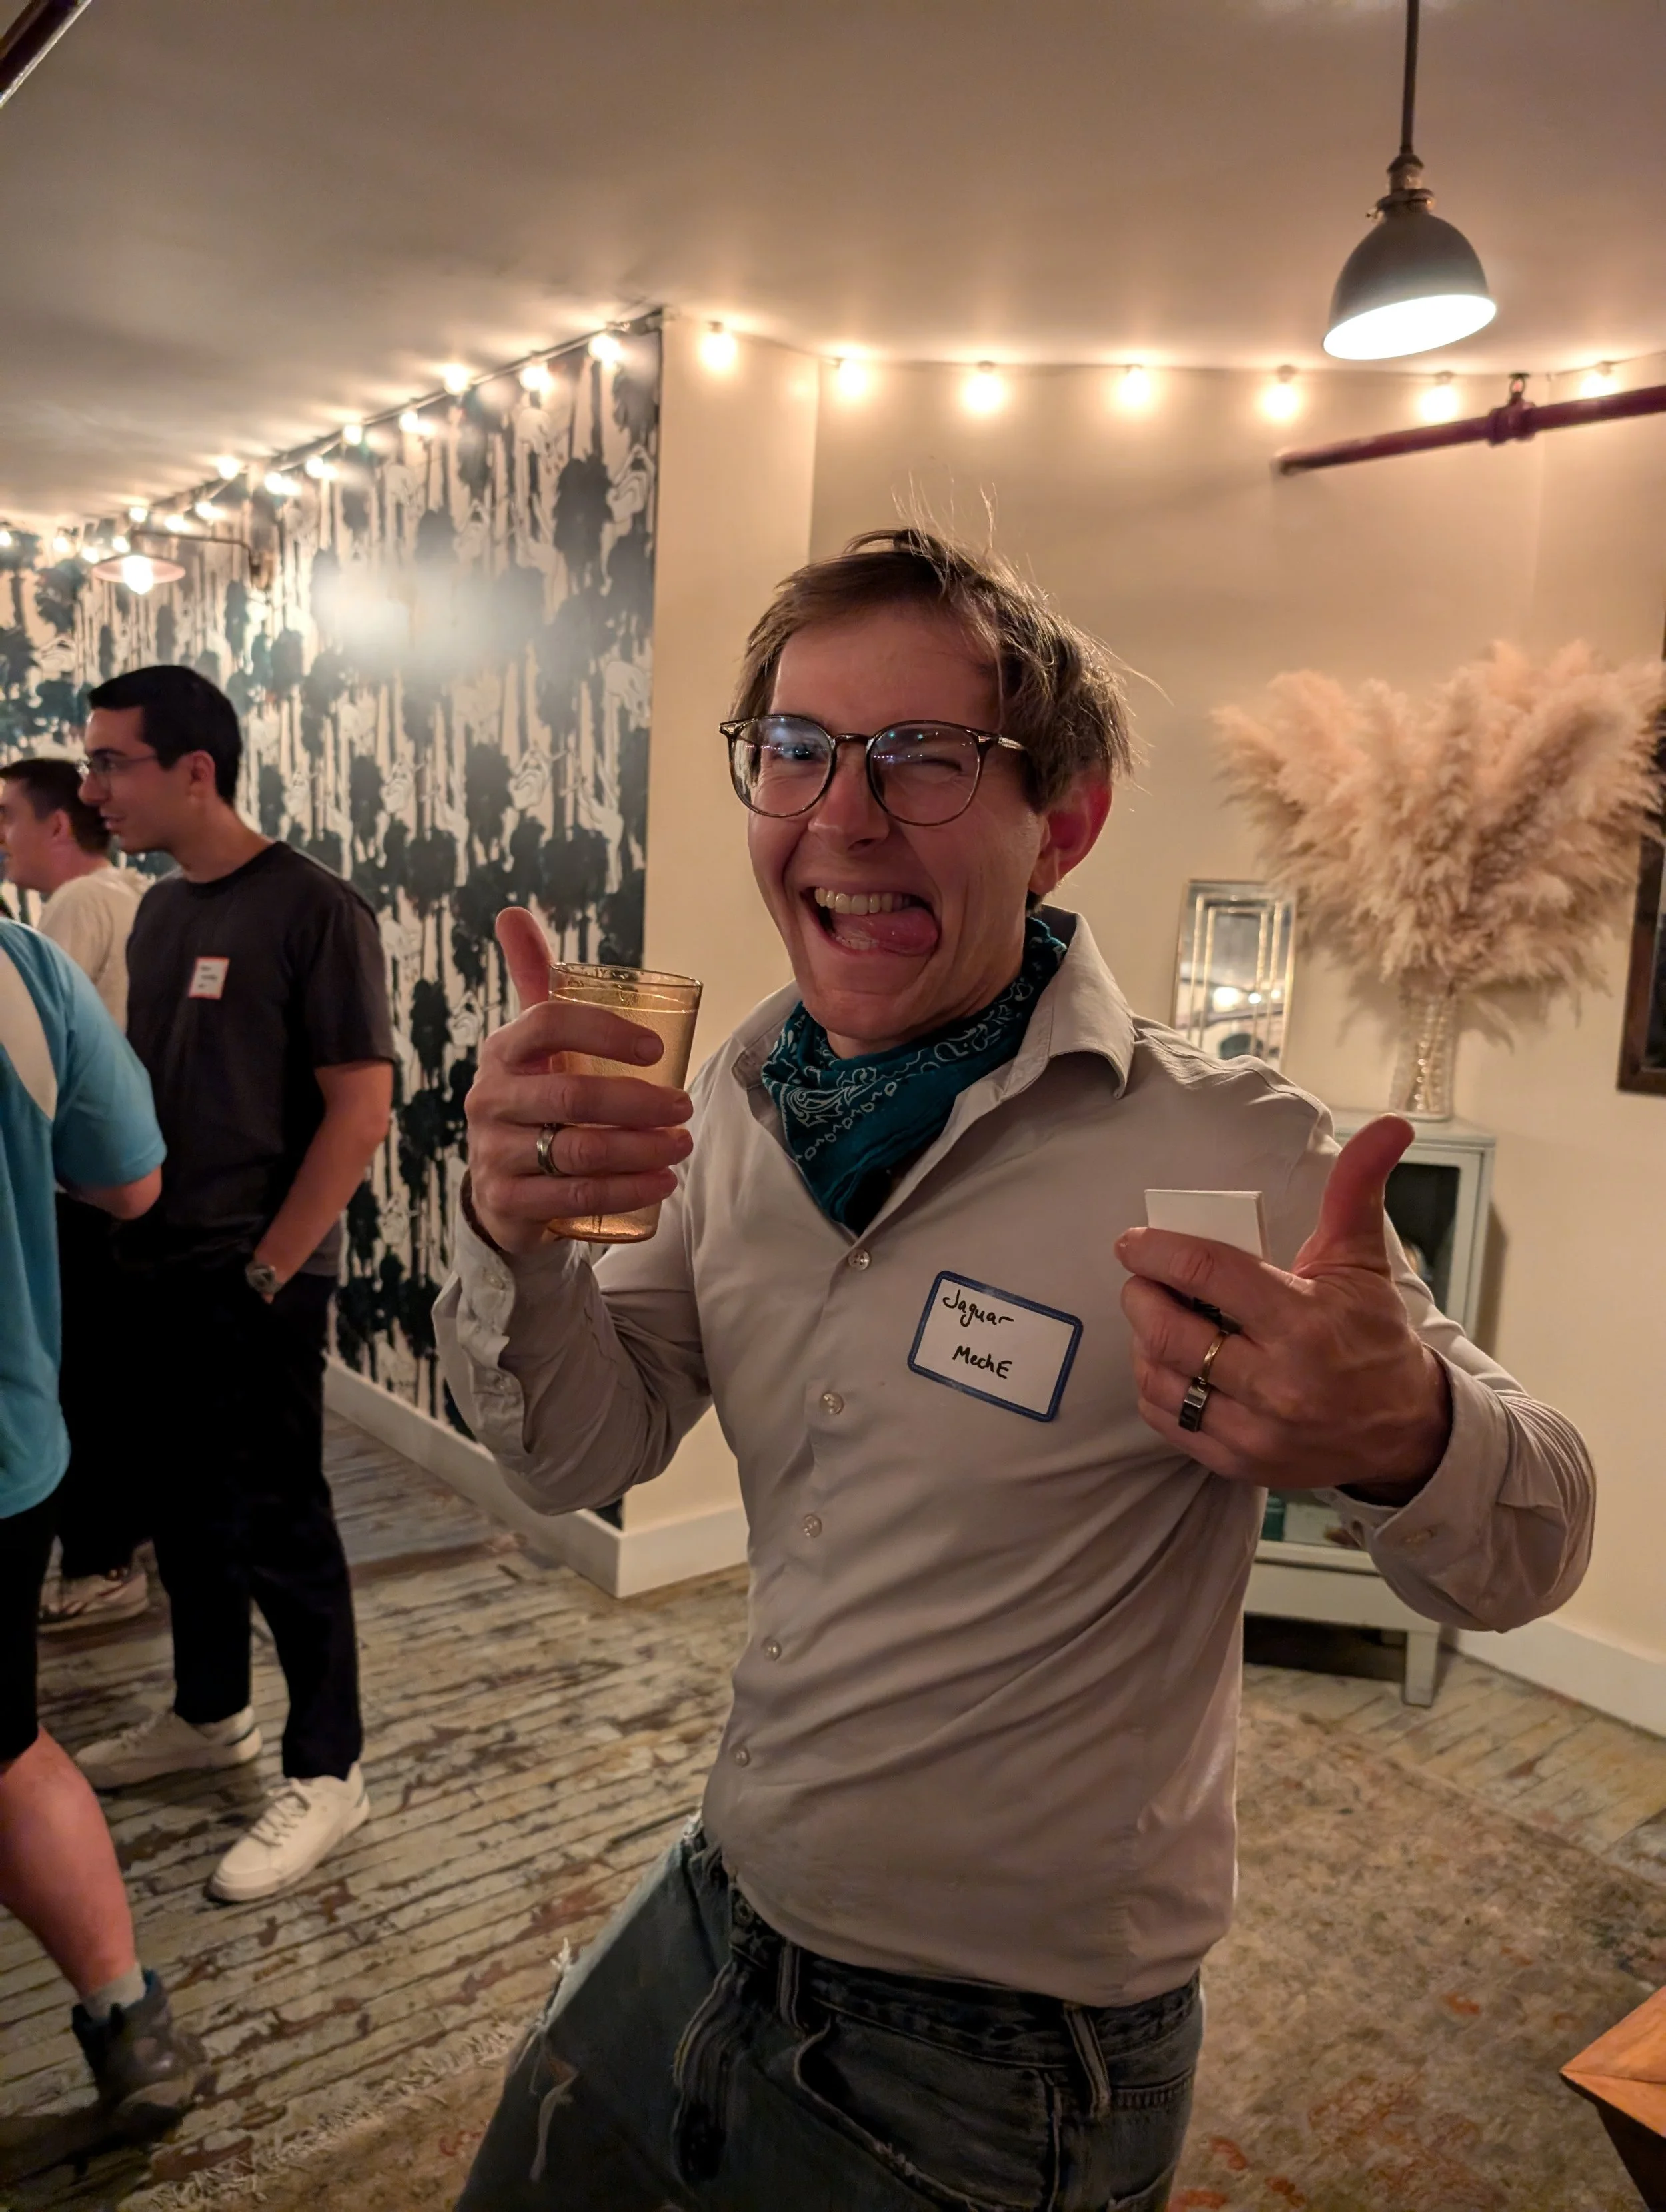
\includegraphics[width=\linewidth,height=23mm,keepaspectratio]{assets/chapters/neuronyc-calendar-meeting.png}
      \par{\tiny NeuroNYC meeting / official event-gallery photo\par}
  \end{columns}
  {\tiny\color{NTXMuted}Sources: \href{https://conorrussomanno.com/}{Conor Russomanno}; \href{https://mathuramg.com/projects/darkMaze.html}{Mathura: Dark Maze}; \href{https://neuro-nyc.org/calendar}{NeuroNYC events / photo}. Historical groups and current organizers are distinct.\par}
  \note{[10:15--11:15] Conor Russomanno dates his NeuroTechNYC organizing to July 2015. Dark Maze was tested at a meetup, documented by Mathura's February 2016 video; the thumbnail is shown above. Neural-network EEG teaching continued in a documented April 2018 Hacknight. The lower photo comes from NeuroNYC's current event gallery; its filename suggests October 2024, but no precise event date is asserted. The newer calendar documents NeuroBall in December 2025, a March 26, 2026 foundation-models symposium and a July 2026 summer summit. The summit calendar header and description disagree on the day, so only the month is used in our source notes. Present this as a continuing city ecosystem, not evidence of a legal merger, rebrand, or current NTX affiliation. The September 10, 2026 Precision Neuroscience careers event remains upcoming at the time of this talk.}
\end{frame}

\begin{frame}{Boston: founders, public dialogue, and community}
  \begin{columns}[c,onlytextwidth]
    \column{.55\textwidth}
      \small
      \NTXPoint{Chapter roots and local founders}{NTX Boston from 2016; Neurable's Ramses Alcaide and Adam Molnar in the local ecosystem.}
      \NTXPoint{2022: public conversation}{Adam joined the NTX Boston / BrainMind neuroethics panel at MIT.}
      \NTXPoint{2025: a successor gathering}{Augmentation Lab's Human Augmentation Summit, August 23, MIT Media Lab: demos, talks, and hands-on exhibits.}
    \column{.41\textwidth}
      \centering
      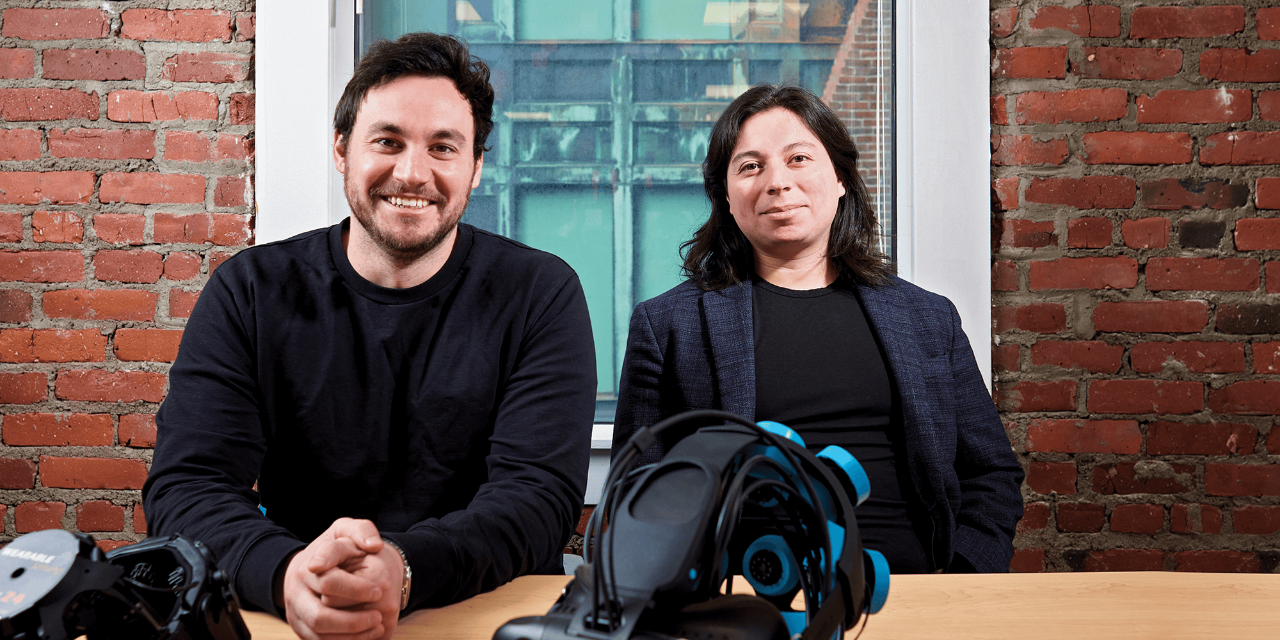
\includegraphics[width=\linewidth,height=22mm,keepaspectratio]{assets/chapters/boston-neurable-founders.png}
      \par{\tiny Adam Molnar (left), Ramses Alcaide (right)\newline Neurable HQ --- Philip Keith Photography / U-M\par}\smallskip
      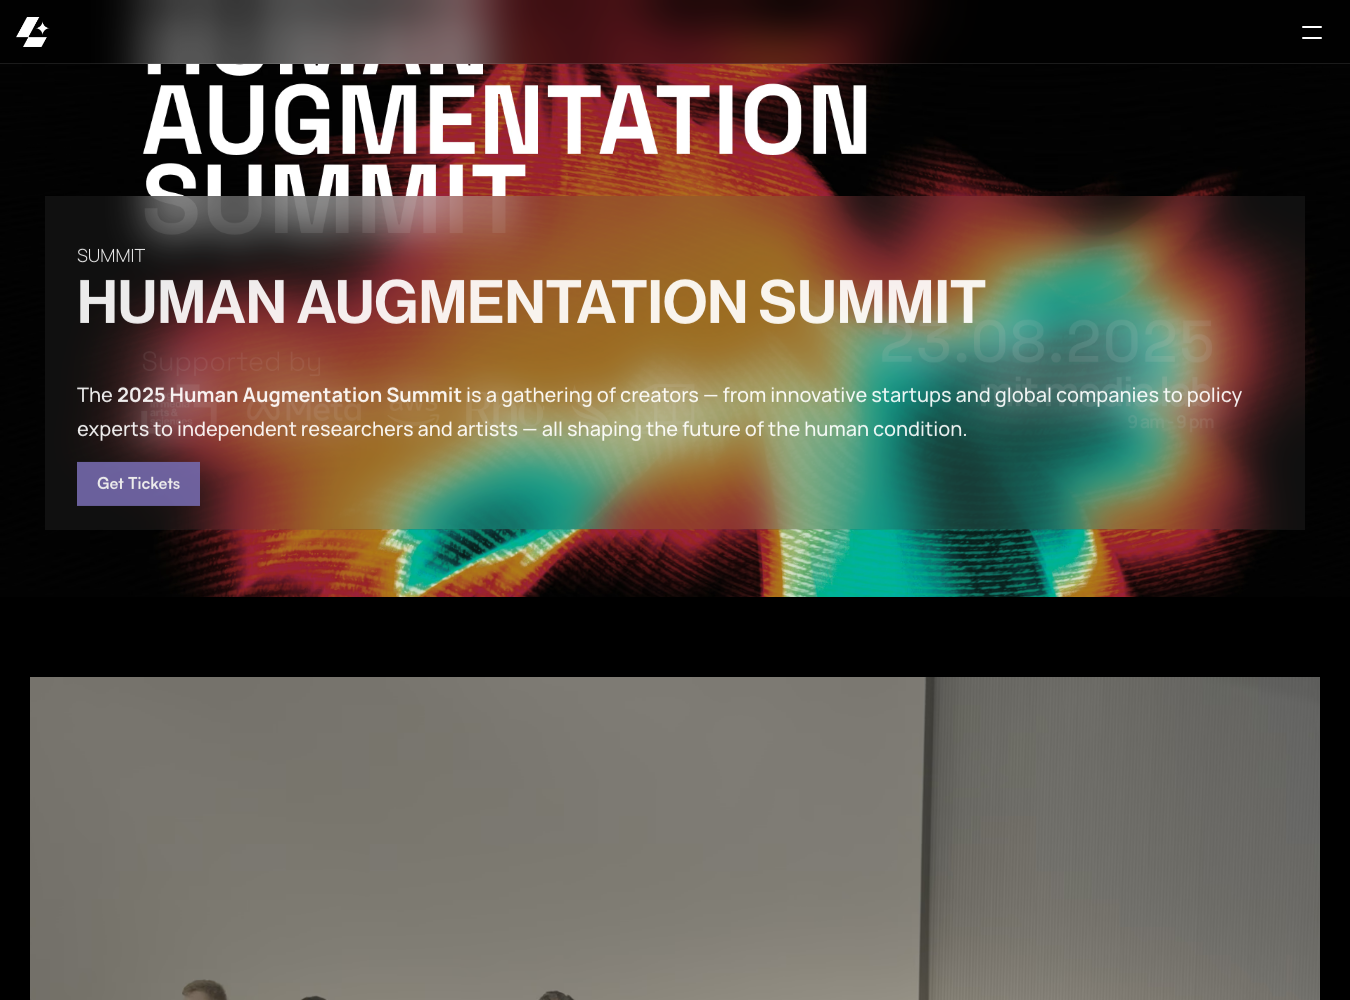
\includegraphics[trim=0 300 0 0,clip,width=\linewidth,height=22mm,keepaspectratio]{assets/history/augmentation-summit-2025-page.png}
      \par{\tiny Official 2025 summit page / Augmentation Lab\par}
  \end{columns}
  {\tiny\color{NTXMuted}Sources: \href{https://neurotechx.com/chapter/1543/}{Boston chapter}; \href{https://www.neurable.com/blog-posts/were-neurable-nice-to-meet-you}{Neurable}; \href{https://augmentationlab.org/summit}{Augmentation Lab summit}. Successor-community framing: Morgan Hough.\par}
  \note{[11:15--12:45] Boston's chapter roots date to 2016. Neurable founders Ramses Alcaide and Adam Molnar are part of the local ecosystem, not established NTX chapter founders. The upper photograph is from U-M's Spring 2023 feature, credited to Philip Keith Photography at Neurable's Boston HQ. Adam joined the June 29, 2022 NTX Boston/BrainMind neuroethics panel at MIT; Alex Higuera was credited for organizing. Morgan identifies Augmentation Lab's 2025 meeting as a successor gathering in this community history. The official page verifies the Human Augmentation Summit on August 23, 2025 at MIT Media Lab in Cambridge, with demos, talks, panels and exhibits. Successor means continuation of local community energy, not an independently verified organizational transfer or NTX ownership. The lower image is the official summit page, not a photograph proving attendance. Boston/London Buzz-in-Review history is retained elsewhere.}
\end{frame}

\begin{frame}{London: connecting research, makers, and students}
  \begin{columns}[c,onlytextwidth]
    \column{.52\textwidth}
      \NTXPoint{May 2016: first meetup at LSE}{With the NERRI project; three-minute talks designed for non-specialists.}
      \NTXPoint{2022: a shared London--Boston event}{Hybrid Buzz-in-Review linked two local communities.}
      \NTXPoint{2025: student-led building}{London Neurotech Hackathon with Imperial's Neurotech Society and partners including NeuroTechX.}
    \column{.43\textwidth}
      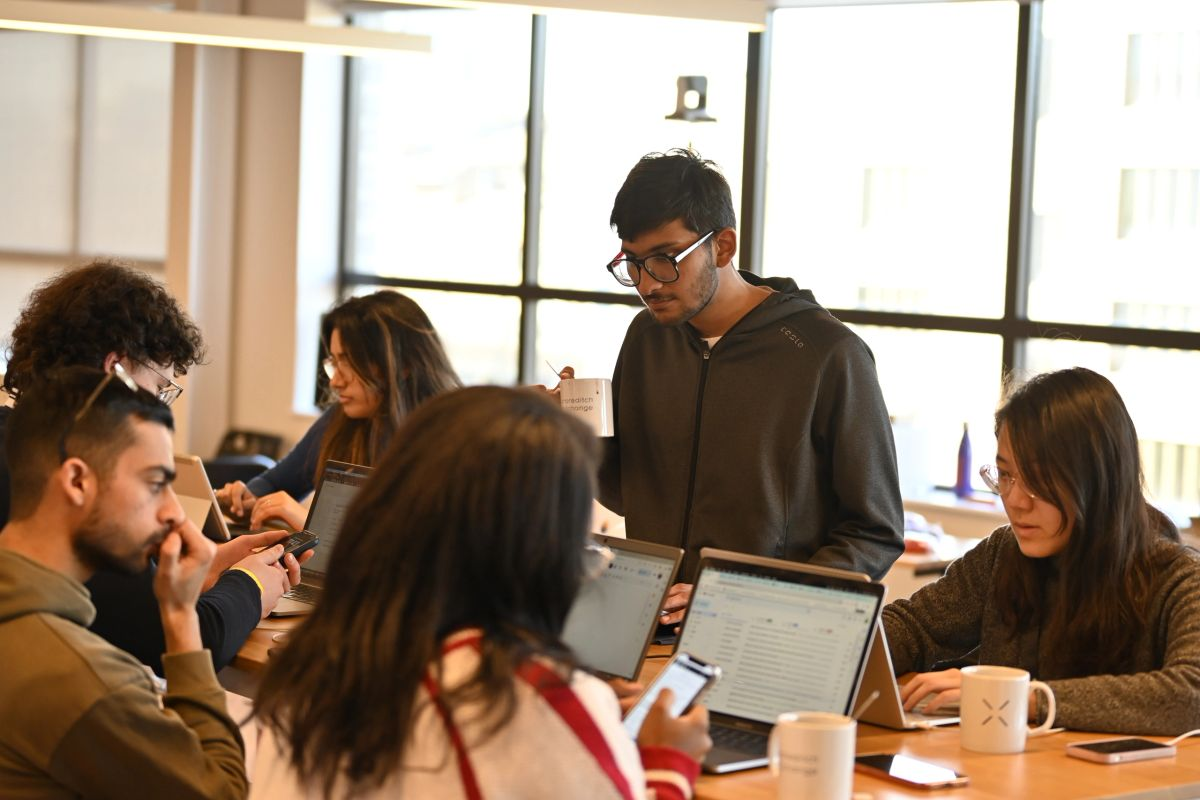
\includegraphics[width=\linewidth,height=43mm,keepaspectratio]{assets/chapters/london-hackathon-2025.jpg}
      \par\smallskip{\scriptsize London Neurotech Hackathon, January 2025\par Photo: Imperial College Neurotech Society\par}
  \end{columns}
  {\tiny\color{NTXMuted}Sources: \href{https://www.meetup.com/NeuroTechLDN/events/230512143/}{May 6, 2016 meetup}; \href{https://www.linkedin.com/posts/ben-woodington_neurotechx-ldn-bos-buzz-in-review-2022-activity-6894574014426398720-_Ash}{2022 organizer announcement}; \href{https://iclneurotech.co.uk/hackathon}{2025 organizer recap / photo}\par}
  \note{[12:45--13:45] The original Meetup listing identifies May 6, 2016 at LSE's New Academic Building as the first London chapter meetup, supported by the NERRI project. Hosts were Javier Asensio and Imre Bard. Its flash-talk format explicitly invited accessible introductions for non-academics, with research, startups, Cybathlon, and London Hackspace Brain Hackers represented. Ben Woodington's announcement describes a February 5, 2022 hybrid Buzz-in-Review shared with Boston, with London's in-person gathering at Bellavita Academy. The image is from Imperial College Neurotech Society's January 25--26, 2025 hackathon recap, which explicitly credits NeuroTechX among its partners. It is not a photograph of the 2016 or 2022 meeting. Avoid the conflicting 30/36-hour descriptions and unverified first-ever superlatives. The thread is continuity through collaborations between local organizers, researchers, makers, and students.}
\end{frame}

\begin{frame}{India: building community across distance}
  \begin{columns}[c,onlytextwidth]
    \column{.58\textwidth}
      \NTXPoint{October 2020: Neuro 2.0}{A two-day online forum connecting the India community with international speakers.}
      \NTXPoint{January 2021: shared Buzz-in-Review}{India and Australia paired in the global chapter program.}
      \NTXPoint{September 2021: India's own ecosystem}{A discussion with Eywa Neuro on invasive BMI, microelectrodes, and bioMEMS manufacturing.}
    \column{.35\textwidth}
      \centering
      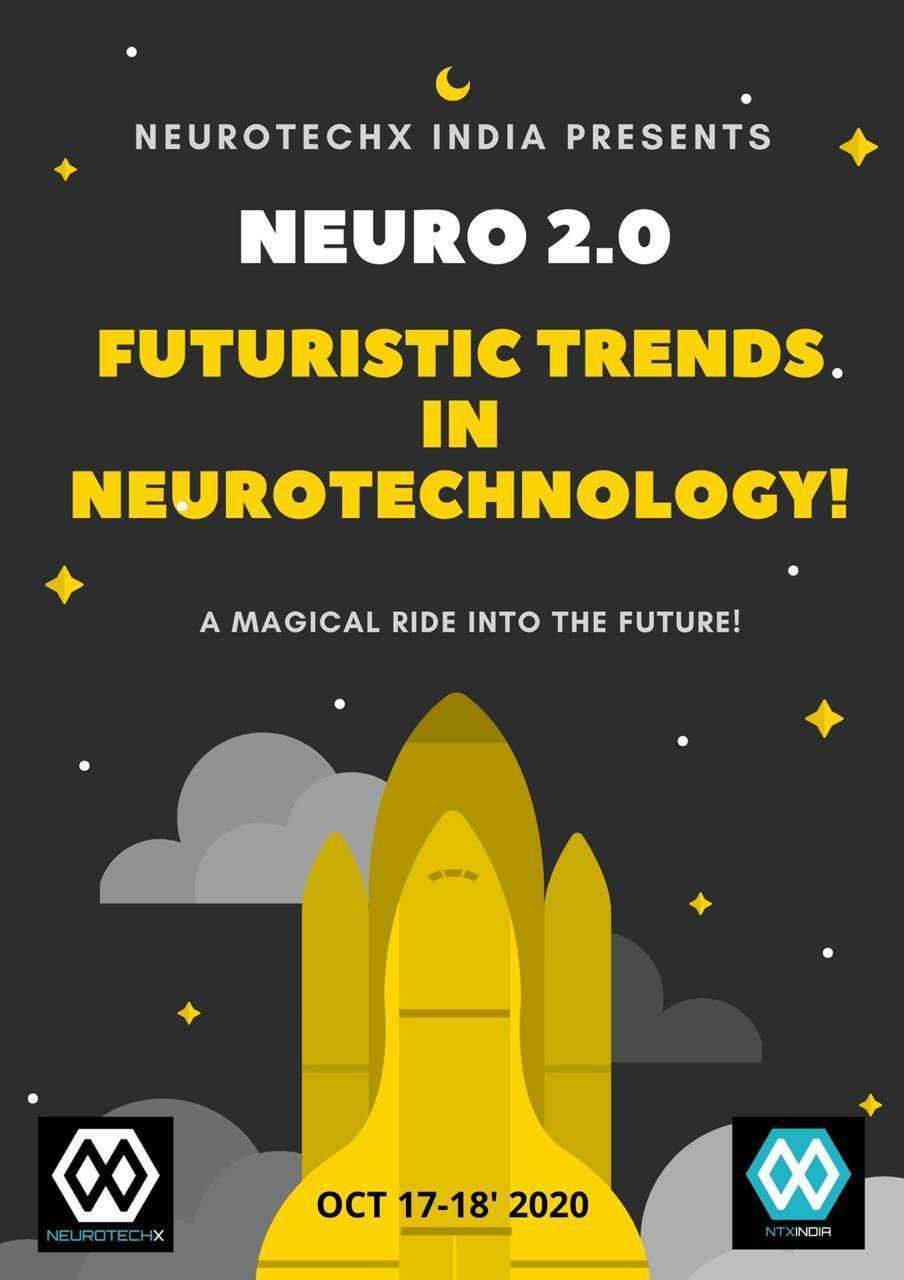
\includegraphics[width=\linewidth,height=46mm,keepaspectratio]{assets/chapters/india-neuro2-2020.jpg}
      \par\smallskip{\scriptsize Original NeuroTechX India event poster\par October 17--18, 2020\par}
  \end{columns}
  {\tiny\color{NTXMuted}Sources: \href{https://neurostars.org/t/neuro-2-0-futuristic-trends-in-neurotechnology/16962}{Neuro 2.0 announcement / poster}; \href{https://neurotechx.com/ntxbir2021/}{Buzz-in-Review 2021}; \href{https://eywaneuro.com/news}{Eywa Neuro: September 4, 2021 talk}\par}
  \note{[13:45--14:45] India is a country-wide community here, not a single city chapter. Neuro 2.0 ran online October 17--18, 2020. The original event artwork and announcement survive on Neurostars; speaker Pia Tikka's university research-group archive independently documents her participation alongside Isabella Pasqualini and David Eagleman on day two. The January 23, 2021 Buzz-in-Review program paired India and Australia. Eywa Neuro's own news archive records Kaustubh's invited September 4, 2021 NTX India talk on invasive BMI, microelectrodes, and India's role in bioMEMS manufacturing. These are documented milestones, not an asserted founding date or claims about attendance. The poster represents an online event, not evidence of an in-person gathering. The lesson is that a geographically distributed community can connect global expertise with local researchers and founders.}
\end{frame}
